%%
%% This is file `sample-sigconf.tex',
%% generated with the docstrip utility.
%%
%% The original source files were:
%%
%% samples.dtx  (with options: `sigconf')
%% 
%% IMPORTANT NOTICE:
%% 
%% For the copyright see the source file.
%% 
%% Any modified versions of this file must be renamed
%% with new filenames distinct from sample-sigconf.tex.
%% 
%% For distribution of the original source see the terms
%% for copying and modification in the file samples.dtx.
%% 
%% This generated file may be distributed as long as the
%% original source files, as listed above, are part of the
%% same distribution. (The sources need not necessarily be
%% in the same archive or directory.)
%%
%%
%% Commands for TeXCount
%TC:macro \cite [option:text,text]
%TC:macro \citep [option:text,text]
%TC:macro \citet [option:text,text]
%TC:envir table 0 1
%TC:envir table* 0 1
%TC:envir tabular [ignore] word
%TC:envir displaymath 0 word
%TC:envir math 0 word
%TC:envir comment 0 0
%%
%%
%% The first command in your LaTeX source must be the \documentclass
%% command.
%%
%% For submission and review of your manuscript please change the
%% command to \documentclass[manuscript, screen, review]{acmart}.
%%
%% When submitting camera ready or to TAPS, please change the command
%% to \documentclass[sigconf]{acmart} or whichever template is required
%% for your publication.
%%
%%
\documentclass[sigconf]{acmart}

%%
%% \BibTeX command to typeset BibTeX logo in the docs
\AtBeginDocument{%
  \providecommand\BibTeX{{%
    Bib\TeX}}}

%% Rights management information.  This information is sent to you
%% when you complete the rights form.  These commands have SAMPLE
%% values in them; it is your responsibility as an author to replace
%% the commands and values with those provided to you when you
%% complete the rights form.
\setcopyright{acmcopyright}
\copyrightyear{2018}
\acmYear{2018}
\acmDOI{XXXXXXX.XXXXXXX}

%% These commands are for a PROCEEDINGS abstract or paper.
\acmConference[Conference acronym 'XX]{Make sure to enter the correct
  conference title from your rights confirmation emai}{June 03--05,
  2018}{Woodstock, NY}
%%
%%  Uncomment \acmBooktitle if the title of the proceedings is different
%%  from ``Proceedings of ...''!
%%
%%\acmBooktitle{Woodstock '18: ACM Symposium on Neural Gaze Detection,
%%  June 03--05, 2018, Woodstock, NY}
\acmPrice{15.00}
\acmISBN{978-1-4503-XXXX-X/18/06}


%%
%% Submission ID.
%% Use this when submitting an article to a sponsored event. You'll
%% receive a unique submission ID from the organizers
%% of the event, and this ID should be used as the parameter to this command.
%%\acmSubmissionID{123-A56-BU3}

%%
%% For managing citations, it is recommended to use bibliography
%% files in BibTeX format.
%%
%% You can then either use BibTeX with the ACM-Reference-Format style,
%% or BibLaTeX with the acmnumeric or acmauthoryear sytles, that include
%% support for advanced citation of software artefact from the
%% biblatex-software package, also separately available on CTAN.
%%
%% Look at the sample-*-biblatex.tex files for templates showcasing
%% the biblatex styles.
%%

%%
%% The majority of ACM publications use numbered citations and
%% references.  The command \citestyle{authoryear} switches to the
%% "author year" style.
%%
%% If you are preparing content for an event
%% sponsored by ACM SIGGRAPH, you must use the "author year" style of
%% citations and references.
%% Uncommenting
%% the next command will enable that style.
%%\citestyle{acmauthoryear}


%%
%% end of the preamble, start of the body of the document source.
\begin{document}

%%
%% The "title" command has an optional parameter,
%% allowing the author to define a "short title" to be used in page headers.
\title{Ideas from the Synthesis Kernel in Modern Systems: Optimization techniques and SuperOptimizers}

%%
%% The "author" command and its associated commands are used to define
%% the authors and their affiliations.
%% Of note is the shared affiliation of the first two authors, and the
%% "authornote" and "authornotemark" commands
%% used to denote shared contribution to the research.
\author{Sridhara Madhu Mohan Nelemane}
\affiliation{%
 \institution{University of Bamberg}
 \city{Bamberg}
 \country{Germany}}

%%
%% By default, the full list of authors will be used in the page
%% headers. Often, this list is too long, and will overlap
%% other information printed in the page headers. This command allows
%% the author to define a more concise list
%% of authors' names for this purpose.
\renewcommand{\shortauthors}{Trovato et al.}

%%
%% The abstract is a short summary of the work to be presented in the
%% article.
\begin{abstract}

    The paper from Henry Massalin \cite{synthesis92} was considered futuristic 
    for its time. Several ideas were proposed in this paper towards developing
    a much more sophisticated operating system. These ideas particularly focussed 
    on performance of the operating system and an implementation called Synthesis
    kernel was used to drive the concept home. This seminar paper refers to the 
    same research and implementation and tries to provide an understanding
    some of the same ideas in the modern context. In particular the paper focuses on
    techniques of SuperOptimization utilized in Runtime Code Generation phase
    of the Synthesis Operating system. 

\end{abstract}

%%
%% The code below is generated by the tool at http://dl.acm.org/ccs.cfm.
%% Please copy and paste the code instead of the example below.
%%
\begin{CCSXML}
<ccs2012>
 <concept>
  <concept_id>10010520.10010553.10010562</concept_id>
  <concept_desc>Operating Systems Design</concept_desc>
  <concept_significance>500</concept_significance>
 </concept>
 <concept>
  <concept_id>10010520.10010575.10010755</concept_id>
  <concept_desc>Optimization</concept_desc>
  <concept_significance>300</concept_significance>
 </concept>
 <concept>
  <concept_id>10010520.10010553.10010554</concept_id>
  <concept_desc>SuperOptimization</concept_desc>
  <concept_significance>100</concept_significance>
 </concept>
 <concept>
  <concept_id>10003033.10003083.10003095</concept_id>
  <concept_desc>Synthesis Kernel</concept_desc>
  <concept_significance>100</concept_significance>
 </concept>
 <concept>
  <concept_id>10003033.10003083.10003095</concept_id>
  <concept_desc>Runtime Code Generation</concept_desc>
  <concept_significance>100</concept_significance>
 </concept>
</ccs2012>
\end{CCSXML}

\ccsdesc{Operating Systems Design-Performance}
\ccsdesc{Optimization - Techniques}
\ccsdesc{SuperOptimization}
\ccsdesc{Synthesis Kernel}
\ccsdesc{Runtime Code Generation}

%%
%% Keywords. The author(s) should pick words that accurately describe
%% the work being presented. Separate the keywords with commas.
\keywords{datasets, neural networks, gaze detection, text tagging}
%% A "teaser" image appears between the author and affiliation
%% information and the body of the document, and typically spans the
%% page.
%%\begin{teaserfigure}
%%  \includegraphics[width=\textwidth]{sampleteaser}
%%  \caption{Seattle Mariners at Spring Training, 2010.}
%%  \Description{Enjoying the baseball game from the third-base
%%  seats. Ichiro Suzuki preparing to bat.}
%%  \label{fig:teaser}
%%\end{teaserfigure}

%%
%% This command processes the author and affiliation and title
%% information and builds the first part of the formatted document.
\maketitle

\section{Introduction}
Before the invention of hyperthreading and powerful processors with big working memories as we have today, the processors had meagre processing power and very low RAM capacity. In such processors, running complex algorithms were challenging. Operating system itself consumed significant resources and optimization was one of the key research topics for operating system experts. It was under these circumstances that Henry Massalin proposed ideas for Operating system optimization. These ideas are extremely relevant even today. However, it needs some investigation with a modern perspective as demonstrated in the blog \cite{synthesis2019}

The paper introduced the concept of Runtime Code generation helping build purposefully optimized code. The techniques included among other ideas, constant folding, constant propagation, and procedure inlining. The paper also proposed the idea of superoptimizer which searches for the smallest of possible programs to achieve a given objectives. These and other ideas are explored in later sections of this paper.

\section{Synthesis Kernel and Operating Systems Design}
The basic premise of the Synthesis kernel proposed in \cite{synthesis92} is that operating system performance can be enhanced through few strategies of optimization during runtime code-generation. Instead of static code, runtime code generation provides an opportunity to dynamically add optimizations in code based on runtime conditions of the system.

\subsection{Key concept and Ideas for performance enhancement}

The paper \cite{synthesis92} introduces run time code generation to optimize kernel performance. The technique benefits from more information regarding the execution and the environment during runtime. 

\subsection{Runtime Code generation and Optimization}
\begin{itemize}
\item{Runtime Code Generation}
\end{itemize}

\section{Traditional Optimization Strategies}
This section revisits some of the traditional optimization strategies at the level of Assembly language to fully utilize processor capabilities. Most general purpose and specialized processors implement multi-stage instruction pipelines. The most common issue in the pipelines is pipeline stalls. This happens when an instruction has to wait for another instruction to pass a certain stage. For example, a Mov instruction waits for the previous Add instruction to write to the register which is used in the Mov instruction. Several optimization techniques are deviced to avoid such stalls. 

\begin{figure}[h]
  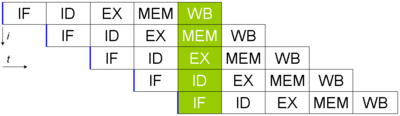
\includegraphics[width=0.45\textwidth]{images/pipelines}
  \caption{Wikipedia, the free encyclopedia, “Atomic force microscopy,” https://en.wikipedia.org/wiki/File:Fivestagespipeline.png}
  \Description{Stages for instruction queue in common processors}
\end{figure}


\subsection{Avoid Decision statements}

Conditional statements like 'if....else...' translate in assembly to a set of JMP instructions. The JMP instructions require a few additional steps like storing the current Program Counter and updating the Stack Pointer so that the program can resume graceful execution when the control returns to the point from where the JMP was called. These additional steps cost CPU cycles and when possible should be avoided. Several hacks are available to counter these through Arithmetic and Logical operations to obtain results similar to what the conditional statements do. 
In case it is impossible to remove the conditional statements, there should at least be an effort to move the condition statements out of a loop construct so that the overheads related to JMP instruction are not repeated several times. 

Example:
\begin{verbatim}
    int maximum(int a, int b) {
        if (a > b)
            return a;
        else
            return b;
    }
\end{verbatim}
Can be replaced by:
\begin{verbatim}
    int maximum(int a, int b) {
        return -(((b - a) >> 31)*a + ((a - b) >> 31)*b);
    }
\end{verbatim}

Several modern compilers are now capable of replacing such conditional statements with logical and arithmetic instructions.

\subsection{Precompute Constants and Constant Expressions}

Sometimes, code can contain variables that for certain use-cases are not subject to change. Such variables should be eliminated and replaced with constants and constant expressions. For the purpose of clarity, such constants can be implemented using Macros which are computed during compilation. 

\subsection{Procedure Inlining}
Similar to Conditional instructions, procedure calls involves several intermediate steps like storing the program counter, updating the stack pointer and then calling a JMP instruction to the procedure being called and a similar set of steps while returning to the caller. This can be avoided with procedure inlining. Procedure inlining provides an elegant way of structuring the code in a modular fashion while not losing the performance gain by executing the instructions in sequence without the overhead of function call. This is generally accomplished by either a prefix for the procedure definition or an annotation placed before the procedure depending on the type of higher-level language used. 

\subsection{Loop Unrolling}
Loops are often the most compute-intensive sections of the code. Pipeline stalls in loops can be hazardous for the performance of programs since the delay is multiplied by the number of iterations. Hence avoiding pipeline stalls in loops is extremely critical. Loop unrolling is done in three steps:
\begin{enumerate}
\item{Preload registers that are used in computation}
\item{Precompute one sample before the loop begins}
\item{Align compute of older samples with loading of new samples to avoid pipeline stalls}
\end{enumerate}
The method best illustrated in the program below. Note that though this technique optimizes the loop, it is based on the assumption that the processor has enough registers available at this point to be utilized in the loop.

\begin{verbatim}
    Loop :
        load R1,(R6)
        load R2,(R6+1)
        mac R1,R2,R3      //..2 t i c k s
        store R3,(R9)
        add R6,2
        inc R7
    EndLoop
\end{verbatim}

The unrolled version is as below:

\begin{verbatim}
    load R1, (R6)
    load R2, (R6+1)
    add R6, 2
    Loop:  
        load R4, (R6)
        mac R1, R2, R3 ..2ticks
        load R5, (R6+1)
    
        add R6, 2
        store R3, (R9)
    
        load R1,(R6)
        mac R4, R5, R7
        load R2, (R6+1)
    
        add R6, 2
        store R7, (R9)
        inc R9
    Endloop
\end{verbatim}


\subsection{Utilize Special Architecture Capabilities}
Some processors also come with specialized hardware in the form of co-processors, special Multiply-Accumulate units, fast I/O units and others. The compilers may not fully utilize these special facilities provided for the processor. Such handling requires customization of the compilers or disabling compiler optimization and manually modifying sections of code to utilize the capabilities better. For example, most multimedia SOCs provide an additional DSP or a Co-Processor for specialized computation and they can do computations independent of the registers and ALU of the main processors. The compiler may not take advantage of such feature while optimizing and hence require manual intervention by specialist programmers.

In such scenarios, the specialists have advanced knowledge of the Instruction architecture of the processor and the special-purpose processors. They decide on which part of the code shall be executed on the processor and which part would be redirected towards special purpose processors. The special purpose processors could be Signal processors, controllers or just a coprocessor with additional MAC units to enable parallel processing. The programmer can use a switch like \#pragma to separate code that should run on the special purpose processor. In such optimizations, each main processor instruction is coupled with one co-processor instruction that is independent of the main processor instruction and are executed in parallel. 


\section{Superoptimization}

Superoptimization refers to finding the shortest algorithm for a specific function by dynamically analyzing the code generated at runtime. Its a run-time method and takes into account the environment where the program runs and the state of the program at the point of application. The search space is the complete instruction set of the given CPU architecture. The program component that performs this search and modifies the program accordingly is called a "SuperOptimizer". The next few sections focus on understanding the architecture, variants, application and limitations of such superoptimizers.

\subsection{Understanding Superoptimizer}

Superoptimizer as described in \cite{superopt87} uses three stages : 1) Boolean Test, 2) Probabilistic Test and 3) Pruning. Boolean Test simply performs a boolean verification if the given candidate in the search procedure returns the exact same output as expected from the original program. The test generally uses a binary bit-exactness tests to a certain pre-defined set of minterms to conclude the result.
The other two stages are steps taken to reduce the search time. 
Probabilistic test is conducted using a set of test vectors that maximizes the probability that an incorrect program fails thereby reducing the size of the search space. 
Pruning helps further improve search time by filtering out instructions that are obviously redundant. 

\begin{figure}[h]
  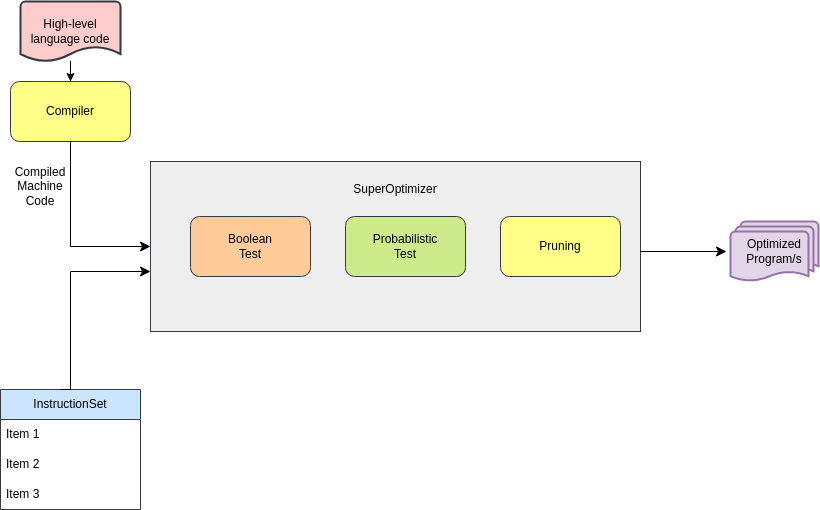
\includegraphics[width=0.45\textwidth]{images/superoptimizer}
  \Description{Basic components of a standard Superoptimizer}
\end{figure}

\subsubsection{Limitations and Applications}
The standard Superoptimizer described above has an obvious limitation that the searched program is limited to the specific architecture. Moreover, in spite of optimizations through probabilistic test and pruning, the search time can be impractical. Another added limitation is that the method does not describe any technique to handle pointers and pointer arithmetics which is a significant part of any system code including kernel. 

Due to these limitations, such a superoptimizer is used in register-based operations, design of RISC architectures and also optimizing little tasks that do not use pointers extensively. Effectively, it can be used as a tool to help assembly language programmers in optimizing the programs and also along with other better superoptimizers \cite{peephole2006} as a preparatory step.

\subsection{Peephole Superoptimizers}

The diagram below (derived from \cite{peephole2006}) shows the components of a Peephole superoptimizer.

\begin{figure}[h]
  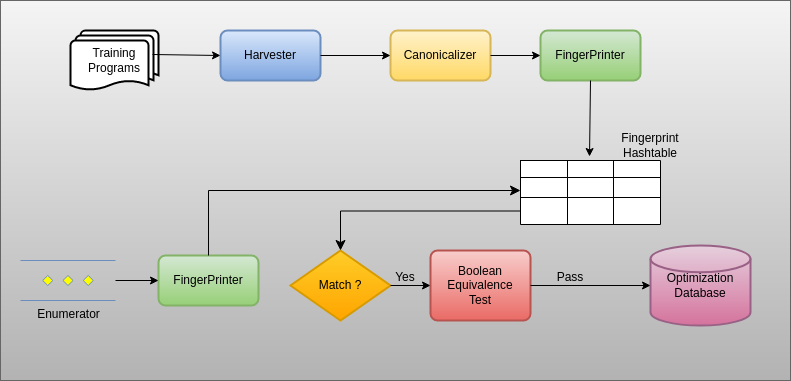
\includegraphics[width=0.45\textwidth]{images/autosuperopt}
  \Description{Architecture of Automatic Peephole Superoptimizer}
\end{figure}

A peephole superoptimizer is basically intend to replace a sequence of instructions with an equivalent faster sequence of instructions. One proposal \cite{peephole2006} uses automatically generated set of pattern-matching rules from a database of thousands to millions of optimizations. The goal with this superoptimizer is to achieve optimizations that are not explored by the compilers and possibly also not found by human optimizers. 

The optimizations are computed offline and fed into a search database which can be accessed over a network instead of storing locally - referred to as network-based search engine. 
The type of instructions considered include loop-free assembly sequence. 

The system to achieve peephole superoptimization has several stages briefly described below:

\subsubsection{Harvester}

This stage considers several reprensentative applications identifying harvestable instruction sequence as target sequences. The choice of the target instruction sequences is based on two constraints - 1) The sequence must have a single entry point and 2) After the first instruction, no other instruction in the sequence should be a jump target (ensuring the 1st condition).   

\subsubsection{Canonicalizer}

In this stage, all instruction sequences that are equivalent to other sequences are filtered out to reduce the number of sequences under consideration. For example, A sequence is said to be \textit{canonicalized} if registers and constants are named in the order of their appearance. 


\subsubsection{FingerPrinter}

Further filtering is done in order to eliminate equivalence. The result of every instruction sequence in the target group is hashed and any instruction sequence that produces a result with a matching hash is eliminated as unnecessary. The hash is also called the \textit{Fingerprint} of the instruction sequence. A hash table is constructed with hashes for all target instruction sequences. The \textit{fingerprint} is an index into the vector of instruction sequences and is provides much faster access compared to instruction sequence search. 

\subsubsection{Enumerator}

A few additional restrictions when applied to the target instruction sequence group, further reduces the search space. These restricted set of instructions are said to be enumerable instruction sequences. An enumerable instruction set is a sequence that has at most two exit points allowing for at most one conditional instruction in a sequence.  The number of distinct registers is restricted to 4 since most instruction sets under 8 instructions per set use less than 4 registers in practice. The number of constants per instruction set as a common practice is reduced to 2. The number of indirect memory access is also reduced by the constraint on the number of registers used. Also the accessible memory is sandboxed and every instruction set is provided with a suitable offset that places all memory accesses within the sandbox territory. These measures though restrictive produces highly efficient superoptimizations and produce quicker results. Such enumeration steps provide exponential performance benefits. 


\subsubsection{Boolean Equivalence Test}

After finding a suitable enumerated instruction sequence from the fingerprint hash table, it is necessary to evaluate the correctness of the sequence. This is achieved through Boolean Equivalance Test. This tests is carried out in two steps: 

\begin{itemize}
\item{\textbf{Execution Test:}}
Run the instruction set over a set of test vectors and compare the results.
\item{\textbf{Boolean Equivalance Test:}}
This test further tests the equivalence accurately using a SAT solver taking into consideration the current the state of the system defined by the values in the registers and the current memory map.
\end{itemize}


\subsubsection{Optimization Database}

The optimizations discovered in the process can be stored into a database which is indexed by the original instruction sequence in its canonical form and the set of live registers. With this database, the steps to optimize a code sequence becomes simpler and involves steps like, harvesting a sequence, canonicalizing it and searching the database to find if an optimization exists. This can be a running database that gets updated if an optimization is not found and is discovered through the longer process. In summary, the database can act as an intermediate cache for optimizations. 

\section{Superoptimizers in Modern Compilers}

The GNU compiler provides a simple Command Line tool that can produce superoptimized code from a set of assembly instructions on a specific architecture. The tool supports several architectures and acts as a helping aid to developers and professional optimizers as an initial step before they carry out more elaborate optimizations. The documentation for this tool is available at \cite{gnu} and can be experimented on any linux distribution. 

SPARC, MC68000, MC68020, M88000, POWER, POWERPC, AM29K, I386, I960 (for i960 1.0), I960B (for I960B 1.1), PYR, ALPHA, HPPA, SH are supported by this tool.

An example usage is depicted below:

\begin{verbatim}

$ make CPU=-D<cpu_name_from_list> superopt
$ superopt -f <goal-function> | -all [-assembly] 
  [-max-cost n] [-shifts] [-extracts] [-no-carry-insns] 
  [-extra-cost n]

\end{verbatim}

As we can see this tool is easy to use and universally available. However, the key limitation of superopt CLI tool is that its too slow. The time complexity of the underlying algorithm is exponential with respect to the instructions on the architecture. Some instructions sets with just 7 instructions might take a week to produce the optimization result. Hence this is still not practical for many use-cases.

Here is an example of working with GNU Superopt. The example generates 6 possible sequences of assmembly instructions for i386 architecture to execute the ABS instruction.

\begin{verbatim}

$ superopt-i386 -fabs -as
Searching for { r = (signed_word) v0 < 0 ? -v0 : v0; }
Superoptimizing at cost 1 2 3 4

1:	movl	%eax,%edx
	sarl	$31,%edx
	addl	%edx,%eax
	xorl	%eax,%edx

2:	movl	%eax,%edx
	sarl	$31,%edx
	addl	%edx,%eax
	xorl	%edx,%eax

3:	movl	%eax,%edx
	sarl	$31,%edx
	xorl	%edx,%eax
	subl	%edx,%eax

4:	movl	%eax,%edx
	sarl	$31,%eax
	addl	%eax,%edx
	xorl	%eax,%edx

5:	movl	%eax,%edx
	sarl	$31,%eax
	addl	%eax,%edx
	xorl	%edx,%eax
	
6:	movl	%eax,%edx
	sarl	$31,%eax
	xorl	%eax,%edx
	subl	%eax,%edx
[6 sequences found]

\end{verbatim}

The max-cost paramater can be set to convey the maximum number of instructions the optimizer can use limiting the number sequences to those that can be executed with this cost. For example, reducing the max-cost for the ABS example above to 3 leads to failure since the superoptimizer cannot find any such sequences.

\begin{verbatim}

$ superopt-i386 -fabs -as -max-cost 3
Searching for { r = (signed_word) v0 < 0 ? -v0 : v0; }
Superoptimizing at cost 1 2 3 failure.

\end{verbatim}

\subsection{A Synthesizing Superoptimizer}

Another effort worth mentioning regarding superoptimizations in modern compilers is described in \cite{souper}. \cite{souper} along with the source at \textit{https://github.com/google/souper} presents a synthesizing superoptimizer that generates optimizations using SMT solvers which generalizes the binary SAT solver to consider real numbers, integers and other data structures including arrays, bit-vectors and more (\cite{SMT}). The superoptimizer was called Souper and was able to work with LLVM and Microsoft Visual C++ compilers.  

TODO: A PRACTICAL SOUPER EXAMPLE HERE

\subsection{Superoptimization of WebAssembly Bytecode}


\section{Other Related Works and Future Direction}

In this paper, the initial works of Massallin \cite{superopt87}, peephole superoptimizers \cite{peephole2006} and the implementations in currenProjectt GNU compilers are presented. In addition to this \cite{denali2001} presents a goal-directed superoptimizer that uses an automatic-theorem prover to generate optimal code for several architectures. The general problem with the superoptimizers has been that the programs generated are relevant to specific processor architectures. Traditional techniques lacked scalability and using them on large programs pose several practical challenges. However, owing to improved computing with the advent of cloud computing and evolution of several statistical techniques including machine learning, have recently provided opportunities to look into superoptimization of programs. Some areas where more research has been carried out and future directions are present here.

\subsection{Applications and Use-cases}

One area that has been explored with superoptimization is enhancing the use-cases where superoptimizers can be applied. Generally used as an aide to professional optimizers and developers, it can be extended if there is a way to apply across multiple architectures. The binary translation using superoptimizer as presented in \cite{BTLpeephole} as a solution to translate optimized assembly from one architecture to another. 

\subsection{Scalability}
These techniques allow for scalable superoptimization. The paper \cite{scaleup} presents an approach presents a search algorithm called LENS that increases the size of the code synthesizable by the superoptimizer. The problem at hand is to search for a program that is semantically equivalent to a given program, but faster according to a specific performance model that uses a set of test cases comprising of test-inputs and test-outputs. The paper \cite{scaleup} models as a graph search problem with each program state represented as a node. The starting node is a set of instructions and the goal node is the optimized equivalent or the target program.

\subsection{Statistical Approaches}

\cite{stochastic}

\subsection{Machine Learning Approaches}

Over the last decade, machine learning and deep learning techniques have made unbelivable advances and have seen use-cases in various fields. It is only but natural, that the domain of systems optimization cannot be left out. A large number of really good code easily accessible from open source repositories creates a huge data set which the authors of \cite{realworld} call \textbf{Big Assembly}. \cite{realworld} describes an approach called SILO (Self Imitation Learning Optimization) that is trained on a subset of the Big Assembly and progressively improve superoptimization ability with this training. 

\cite{realworld}


\section{Conclusions}

Synthesis kernel introduced the concept of runtime code generation and superoptimization to enhance the kernel performance. Some of these concepts are relevant even to this day when applied with the modern approaches and new use-cases can be discovered. 




\bibliographystyle{ACM-Reference-Format}
\bibliography{acmart.bib}

\end{document}